\section{Subspace Clustering}
The main idea of subspace clustering is to identify subspaces of a high dimensional space to allow better clustering than the original (full) space. This is opposed to e.g. PCA, which projects the original space onto a new subspace, which may can be hard to interpret for the user.

Three different density-based subspace clustering algorithms will be discussed. First, the grid-based approach will be discussed, after which the density-based approach will be discussed. Note that, only bottom-up approaches will be considered in this paper.



\subsection{CLIQUE}
The key idea of grid-based subspace clustering is to partition the $\mathcal{S}$ into axis-parallel grid structure starting in 1-dimensional space. The grids forms hyper-rectangular \textit{units} (cells) for which we find the number of points in each. Only the units that exceeds a certain threshold are retained, called \textit{dense units}. Next, adjacent dense units will be merged to form so called \textit{candidate dense units} (CDUs), which will be used to find clusters in higher dimensional subspaces. The goal is then to describe the clusters using a minimal description in the form of DNF (\textit{Disjunctive Normal Form}) expressions.

CLIQUE is a bottom-up, grid-based subspace clustering algorithm that uses the monotonicity property as its clustering criterion, as described in Lemma \ref{lem:mono}.

The proof is provided in \cite{clique}.

The algorithm begins by partitioning the dataset $\mathcal{S}$ into equal-sized intervals (also called windows) of width $\varepsilon$ (input parameter), creating axis-parallel rectangular units. It then scans the dataset to identify 1-dimensional (1D) dense units by counting the number of points in each interval using a histogram, as shown in Figure \ref{fig:dense_cells_and_regions}. For example, with a grid size of $\varepsilon = 0.2$, three intervals in dimension $A_1$ exceed the density threshold $\tau$ (input parameter), while dimension $A_2$ reports four dense units. These dense units are known as \textit{candidate dense units} (CDUs).

The algorithm proceeds incrementally: it starts from 1D and moves to 2D, 3D, and so on, until no more CDUs can be generated. At each stage, the algorithm makes another pass over the dataset to determine which CDUs are dense in the higher dimensions, using the $(k-1)$-dimensional dense units identified in the previous stage. Specifically, CDUs in $k$ dimensions are formed by merging dense units in $(k-1)$ dimensions that share the first $(k-2)$ dimensions. This process continues until no further CDUs are generated.

To optimize performance, CLIQUE applies a pruning technique called \textit{coverage} (from \cite{clique}) to reduce computation time. This technique prunes subspaces with low coverage (i.e., those containing fewer points). However, this may risk eliminating subspaces that could potentially contain clusters.

Once all dense units are identified, CLIQUE defines clusters as maximal sets of connected dense units. For each $k$-dimensional subspace, the algorithm computes disjoint sets of connected dense units, where two units are connected if they share $k-1$ dimensions (a common face in the $k$-dimensional space) or if they are indirectly connected through other units. The algorithm then generates minimal cluster descriptions by covering each set of connected dense units with maximal regions and determining the minimal cover. For instance, in Figure \ref{fig:dense_cells_and_regions}, the minimal cover of the clusters is $A \cup B$, expressed as: $((0.2 \leq A_1 < 0.6) \land (0.4 \leq A_2 < 0.8)) \lor ((0.4 \leq A_1 < 0.8) \land (0.2 \leq A_2 < 0.6))$.
\begin{figure}[H]
    \vspace*{-0.5cm}
    \centering
    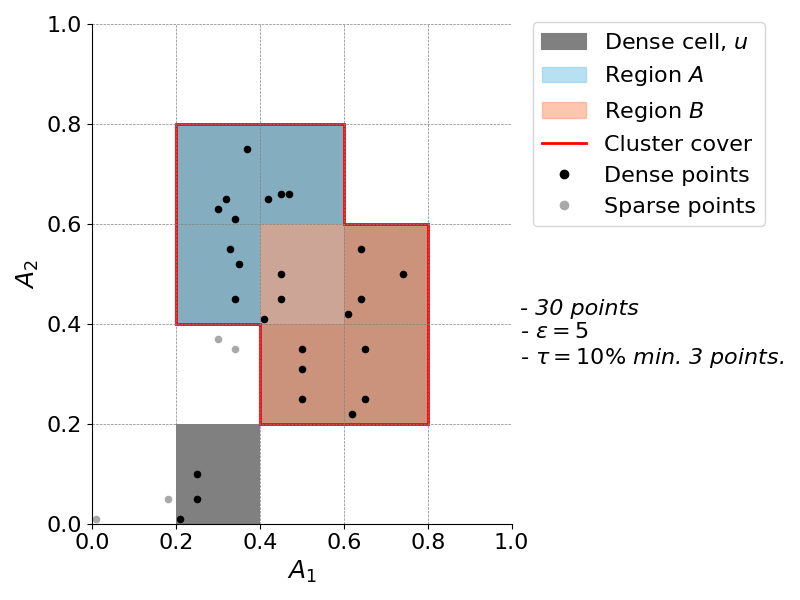
\includegraphics[width=0.4\textwidth]{figures/dense_cells_and_regions.png}
    \caption{Illustration of a dense unit $u$ and two overlapping dense regions $A$ and $B$.}
    \label{fig:dense_cells_and_regions}
    \vspace*{-0.5cm}
\end{figure}

\subsection{MAFIA}
MAFIA is an extension to CLIQUE where the grid sizes are adaptive meaning that the grid sizes are not fixed but are automatically determined by an algorithm. Moreover, the intention is not to rely on user specified input parameters like CLIQUE. In addition, MAFIA do not implement the pruning technique as noted in \cite{clique}, this could result in lost information.

The authors of MAFIA therefore introduces the \textit{Adaptive} algorithm, which starts by divide each dimension into a high number of equal-sized bins -- default it is $n = 1000$ bins. After dividing the dimension into $n$ bins, it merges the bins from left to right. Two bins are merged together if they are within a percentage of difference $\beta$ (input parameter). That means, a high beta value result in many merged bins, and vice-versa. If two bins are merged together, the highest bin count of the two are used to further merge with the next bin. An example is shown in Figure \ref{fig:adaptive_grids}, where in (a) shows the bins before merging and in (b) shows the bins after merging. The result of the algorithm, as can be seen in the figure, is that bins with similar counts are merged together. At last the algorithm determines a so called \textit{threshold-level} for each of the variable-sized bins. The threshold-level is determined by the size of the bin and a so called \textit{cluster dominance factor} $\alpha$ (input parameter). A higher $\alpha$ will result in a higher threshold-level, meaning that the bin must contain more points to be considered a dense unit, and vice-versa.

\begin{figure}[H]
    \vspace*{-0.5cm}
    \centering
    \subfloat[][Uncombined bins]{%
        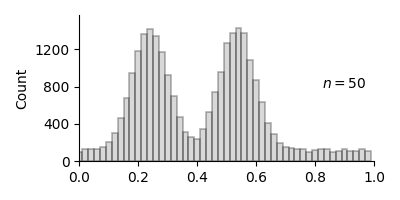
\includegraphics[width=0.4\textwidth]{figures/uncombined_histogram.png}\label{fig:uncombined_bins}}~~~~
    \subfloat[][Combineed bins]{%
        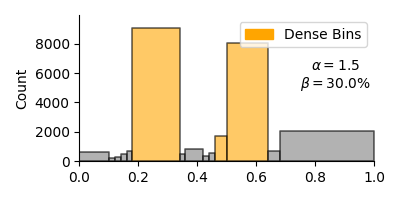
\includegraphics[width=0.4\textwidth]{figures/combined_histogram.png}\label{fig:combined_bins}}~~~~
    \caption{Illustration of the adaptive grids computation.}
    \label{fig:adaptive_grids}
    \vspace*{-0.5cm}
\end{figure}

Having completed the adaptive grid computation, MAFIA proceeds like CLIQUE by scanning the dataset to identify dense units in each subspace. However, the CDUs are generated differently.

\subsubsection{CDU Generation}

\subsection{SUBCLU}
A drawback of grid-based methods is that the quality of clustering depends on the positiong of the grids. In Figure \ref{fig:dense_cells_and_regions}, we see that the due to the rigid grid structure we might miss cluster points, that is point not in a dense cell. This problem especially occurs for clusters that are not of rectangular shapes. In contrast, SUBCLU which extends the principles of DBSCAN to subspaces, that is it relies on the locality assumption of points.

The algorithm starts by identifying clusters in 1-dimensional subspaces, applying DBSCAN to each attribute separately. In this step, it looks for dense regions using a parameter $\epsilon$, which defines the radius within which points are considered neighbors, and $m$, the minimum number of points required for a region to be dense. If clusters are detected in these 1-dimensional subspaces, they are further explored in higher dimensions.

The next phase involves a bottom-up approach where the algorithm combines previously detected $k$-dimensional subspaces that share $k-1$ attributes to generate $(k+1)$-dimensional candidate subspaces. By extending the clusters found in lower-dimensional subspaces, SUBCLU tests if they persist when new dimensions are added. DBSCAN is again applied in these candidate subspaces with the same $\epsilon$ and $m$ values, checking whether clusters detected in the lower-dimensional space still qualify as clusters when higher dimensions are included.

Efficiency is achieved through the monotonicity property of density-connected sets: if no clusters exist in a $k$-dimensional subspace, then higher-dimensional subspaces derived from it will not contain clusters, allowing the algorithm to prune the search space.

For candidate subspaces where clusters are found, SUBCLU further refines these clusters by choosing subspaces with minimal numbers of objects in the clusters, which reduces the computational load when expanding them into higher dimensions.